\documentclass[convert={density=1000,size=300x,outext=.png}]{standalone}

\usepackage{tikz}
\tikzset{>=stealth}

\def\yhat{\hat{y}}

\begin{document}
  \footnotesize
  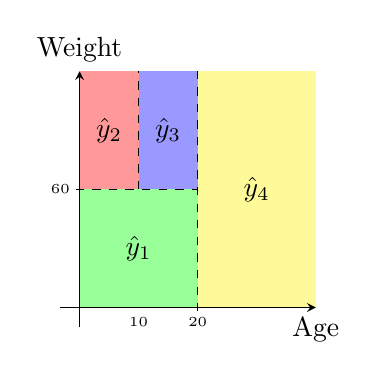
\begin{tikzpicture}
    \fill [green!40] (0,0) rectangle (1.5,1.5) node [black,pos=0.5] {$\yhat_1$};
    \fill [red!40] (0,1.5) rectangle (0.75,3) node [black,pos=0.5] {$\yhat_2$};
    \fill [blue!40] (0.75,1.5) rectangle (1.5,3) node [black,pos=0.5] {$\yhat_3$};
    \fill [yellow!40] (1.5,0) rectangle (3,3) node [black,pos=0.5] {$\yhat_4$};

    \draw [->] (-0.25,0) -- (3,0) node [below] {Age};
    \draw [->] (0,-0.25) -- (0,3) node [above] {Weight};

    \draw [dashed, shorten <= -0.5mm] (1.5,0) node [below] {\tiny $20$} -- (1.5,3);
    \draw [dashed, shorten <= 1.5cm] (0.75,0) node [below] {\tiny $10$} -- (0.75,3);
    \draw [dashed, shorten <= -0.5mm] (0,1.5) node [left] {\tiny $60$} -- (1.5,1.5);
  \end{tikzpicture}
\end{document}
